\documentclass[a4paper]{article}

\usepackage[a4paper,top=0.4in,left=0.4in,right=0.4in,bottom=0.4in]{geometry}
\usepackage{graphicx}
\usepackage{rotating}


\usepackage{setspace}
\usepackage{float}
\graphicspath{ {./images/} }

\usepackage{tabularx,ragged2e,booktabs,caption}
\newcolumntype{C}[1]{>{\Centering}m{#1}}
\renewcommand\tabularxcolumn[1]{C{#1}}

\usepackage{titling}
\setlength{\droptitle}{-10em}

\title{Group Project - 7CCSMGPR \hspace{0.5 cm}Deadline Fighters}
\renewcommand\maketitlehookc{\vspace{-10ex}}

\begin{document}

{\setstretch{0.75}
\begin{center}
    
\includegraphics[scale=1]{images/Logo.png}
\end{center}
\begin{center}
        \Huge{Faculty of Natural \& Mathematical Sciences}\\
		\Huge{Group Project - 7CCSMGPR}
\end{center}
\begin{center}
		\Huge Deadline Fighters \\
		\Large Preliminary report - February 8, 2019 \\
\end{center}
\begin{center}
		\large Sivaranjani Subramanian \\
        \large Ka Hang Jacky Au Yeung \\
        \large Lili Chen \\
        \large Letao Wang \\
        \large Qilin Zhou \\
        \large Georgii Fidarov\\
\end{center}

\newpage
\section{Aim}
Our team, \emph{Deadline Fighters}, aim to develop a multi-host file synchronizer which can:
\begin{itemize}
\item{allow upload and download of files from a central server (hub) through client applications with necessary authorization.}
\item{automatically synchronize changes made by client applications unto the corresponding copy of the file in the server.}
\item{handle all possible conflict/non-conflict scenarios of file synchronization (ie. combinations of Create, Edit, Rename, Delete) involving multiple client applications.}
\item{enable file sychronization through both desktop (all platform) and mobile (Android) clients.}
\end{itemize}

\section{Strategy}
\begin{figure}[H]
	\centering
	\textbf{High level workflow}
	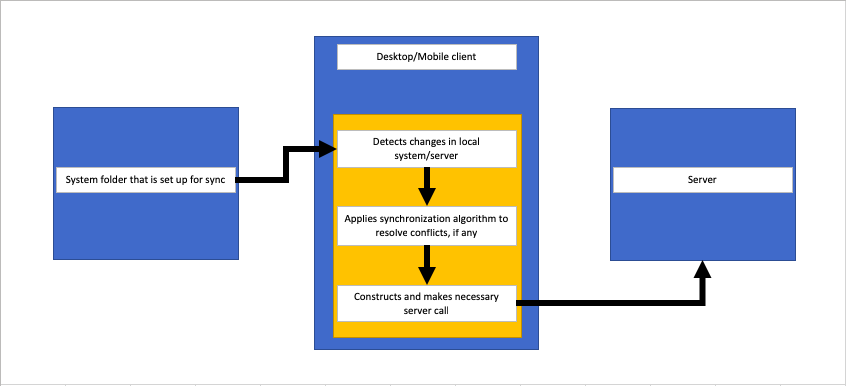
\includegraphics[width=\linewidth]{images/1.png}
	\caption{Flow of control between client and server}
\end{figure}\par
In our Agile workflow, we will start by building a basic prototype of the desktop client. This prototype will perform functionalities of Create, Edit, Rename and Delete for non-conflicting files for single user. It will also have a \emph{Upload} and \emph{Download} button to manually invoke synchronization. Then we will extend this prototype to handle conflict scenarios. The potential conflict scenarios and their resolution are stated in table \ref{table:conflict}.

Once the conflict resolution algorithm implementation is stable, we will develop the mobile client prototype followed by testing conflict resolution using mobile-desktop client pair. After satisfactory testing, we will move to the final phase of introducing automatic file sync using \emph{file system notification} and \emph{server polling}.

\begin{minipage}{\linewidth}
\centering
\captionof{table}{Conflict scenarios and resolutions} \label{table:conflict}
\begin{tabular}[H]{|C{0.75cm}|C{2.25cm}|C{2.25cm}|C{6cm}|}\toprule[1.5pt]
\bf No. & \bf Operation 1 & \bf Operation 2 & \bf Resolution\\\midrule
1       &  Create 	& Create     		&  \begin{flushleft}Upload both files, one with the original name and one with a prefix (eg. (1) or 'copy')\end{flushleft}\\\hline
2       &  Create   & Edit       		&  \begin{flushleft}Upload edit changes to the original file and upload new file with a prefix (eg. (1) or 'copy')\end{flushleft}\\\hline
3       &  Create   & Rename      		&  \begin{flushleft}Rename is applied first followed by upload of new file\end{flushleft}\\\hline
4       &  Create   & Delete     		&  \begin{flushleft}Delete file first and then upload the newly created file\end{flushleft}\\\hline
5       &  Edit		& Edit      		&  \begin{flushleft}Possible strategies: \begin{itemize} \item{Send server error for both requests} \item{Upload two copies of the file, each with different edits} \end{itemize}\end{flushleft}\\\hline
6       &  Edit		& Rename      		&  \begin{flushleft}Rename original file and upload document with edited changes as a new file\end{flushleft}\\\hline
7       &  Edit		& Delete      		&  \begin{flushleft}Delete original file and upload document with edited changes as a new file\end{flushleft}\\\hline
8       &  Rename   & Rename      		&  \begin{flushleft}Rename original file on server to name1 and upload another copy of the file with name2\end{flushleft}\\\hline
9       &  Rename   & Delete      		&  \begin{flushleft}Delete original file and upload another copy of the file with the new name\end{flushleft}\\\hline
10      &  Delete   & Delete      		&  \begin{flushleft}No conflict\end{flushleft}\\
\bottomrule[1.25pt]
\end {tabular}\par
\bigskip
\emph{Operation 1 and 2 are performed on/for files with the same name by same/different users from different devices.}
\end{minipage}

\section{Tools/Technology}
At first, we use GitHub for code hosting, GitHub is a hosting platform for open source and proprietary software projects. It benefits for the team work projects because every member in the team can modify code and pull requests.\\\\
We need to write documents use LaTex , Overleaf is an online LaTex editor that we make use of.\\\\
Before coding, we apply Mockingbot to design user interface and set standards for what the clients will look like.\\\\
For the server, we use Amazon S3, it is a simple cloud storage service. The main reason we use that instead of virtual machine is security, Amazon S3 uses the Advanced Encryption Standard for 256 bits, AES can quickly encrypt and decrypt in software and hardware. When accessKeyID and secretKeyID are exposed to public, the Amazon S3 will send an email to user.\\\\
For the desktop client, we plan to use JavaScript/html/CSS language and the editor is Visual studio code. The structure we use is electron because it integrates \emph{Chromium} and \emph{Node.js} very well together, interfaces and algorithms can be combined in an orderly manner.\\\\
For the mobile client, we use Java on Android studio platform. And for the database, we use Structured Query Language on MySQL.\\\\
At the step of web debugging, we decide to use Charles. Charles is a HTTP proxy server, when the users send requests to server or get responses from server, Charles can monitor all data.\\\\
Testing is a critical part, we decide to use unit test and we preliminarily use Mocha and Junit. Mocha is a testing tool for JavaScript, it is more flexible than other test frameworks. Junit is the most basic testing structure for Java, we should apply it to test mobile client.



\section{Team protocol}
The main method the team choose is that agile software developing, which means that the development is iterative and step-by-step. The project divided into several individual small projects and during developing these small projects, it goes through the requirement, plan, design, development, tests, deploy, review and then go to the next small project.\\\\
There are two types of meeting that the team will be held. The first type is held every week which all members should attend. During this meeting all the team members review the work done last week finding the potential problems and planning for the next week. It usually lasts for 1 hour.\\\\
The other type is held between 1-2 days and this is not for all members but between the members who have the same tasks assigned from last week. This meeting usually does not involve the decision making but the attendance review what they have do after last daily meeting. It lasts for not longer than 5 minutes.\\\\
All team members should push at least one commit every two days. Once a member pulls request on the git, at least 2 members should view changes and approve before it merges on the master branch of the repository. If some members request changes, the member who pulls request should be fixed or give a satisfactory explanation to these changes.



\section{What we have done within recent weeks}
Totally we have 10 meetings within 2 weeks. We have the first meeting to know each other after the team members are allocated and discussed the group name and choose the team coordinator and registered to the GitHub by using Git as required. Analysed what should be achieved in the final and distributed task to each member to looking through the details about the server, unite test, mobile development, desktop development, file sync and conflict resolution on the second meeting. \\\\
After that, we make decisions of each section within a day. We choose to use electron framework to develop the desktop application and java to develop the Android application. Start working with Amazon AWS as service and make it work within a day in the next meeting. \\\\
On the next several meeting, we start working with the electron to develop the desktop application and achieve the upload file function. Also, designed a user interface of the desktop application by using MockingBot. \\\
To start working the initial report, we arrange a meeting to analyse the initial report requirement and make a full plan over the whole development process and distribute into 6 sections to members to working with.

\medskip

\begin{thebibliography}{9}
\bibitem{GitHub}
GitHub, [online]Available at:
\texttt{https://github.com/}(Accessed: 3 February 2019).

\bibitem{ElectronJS}
ElectronJS, [online]Available at:
\texttt{https://electronjs.org/}(Accessed: 3 February 2019).

\bibitem{Amazon S3}
Amazon S3, [online]Available at:
\texttt{https://aws.amazon.com/free/storage/?nc1=h\_ls}(Accessed: 3 February 2019).

\bibitem{Charles}
Charles, [online]Available at:
\texttt{https://www.charlesproxy.com/}(Accessed: 3 February 2019).

\bibitem{Mocha}
Mocha, [online]Available at:
\texttt{https://mochajs.org/}(Accessed: 3 February 2019).

\bibitem{Junit}
Junit, [online]Available at:
\texttt{https://junit.org/junit5/}(Accessed: 3 February 2019).


\end{thebibliography}

\begin{sidewaysfigure}
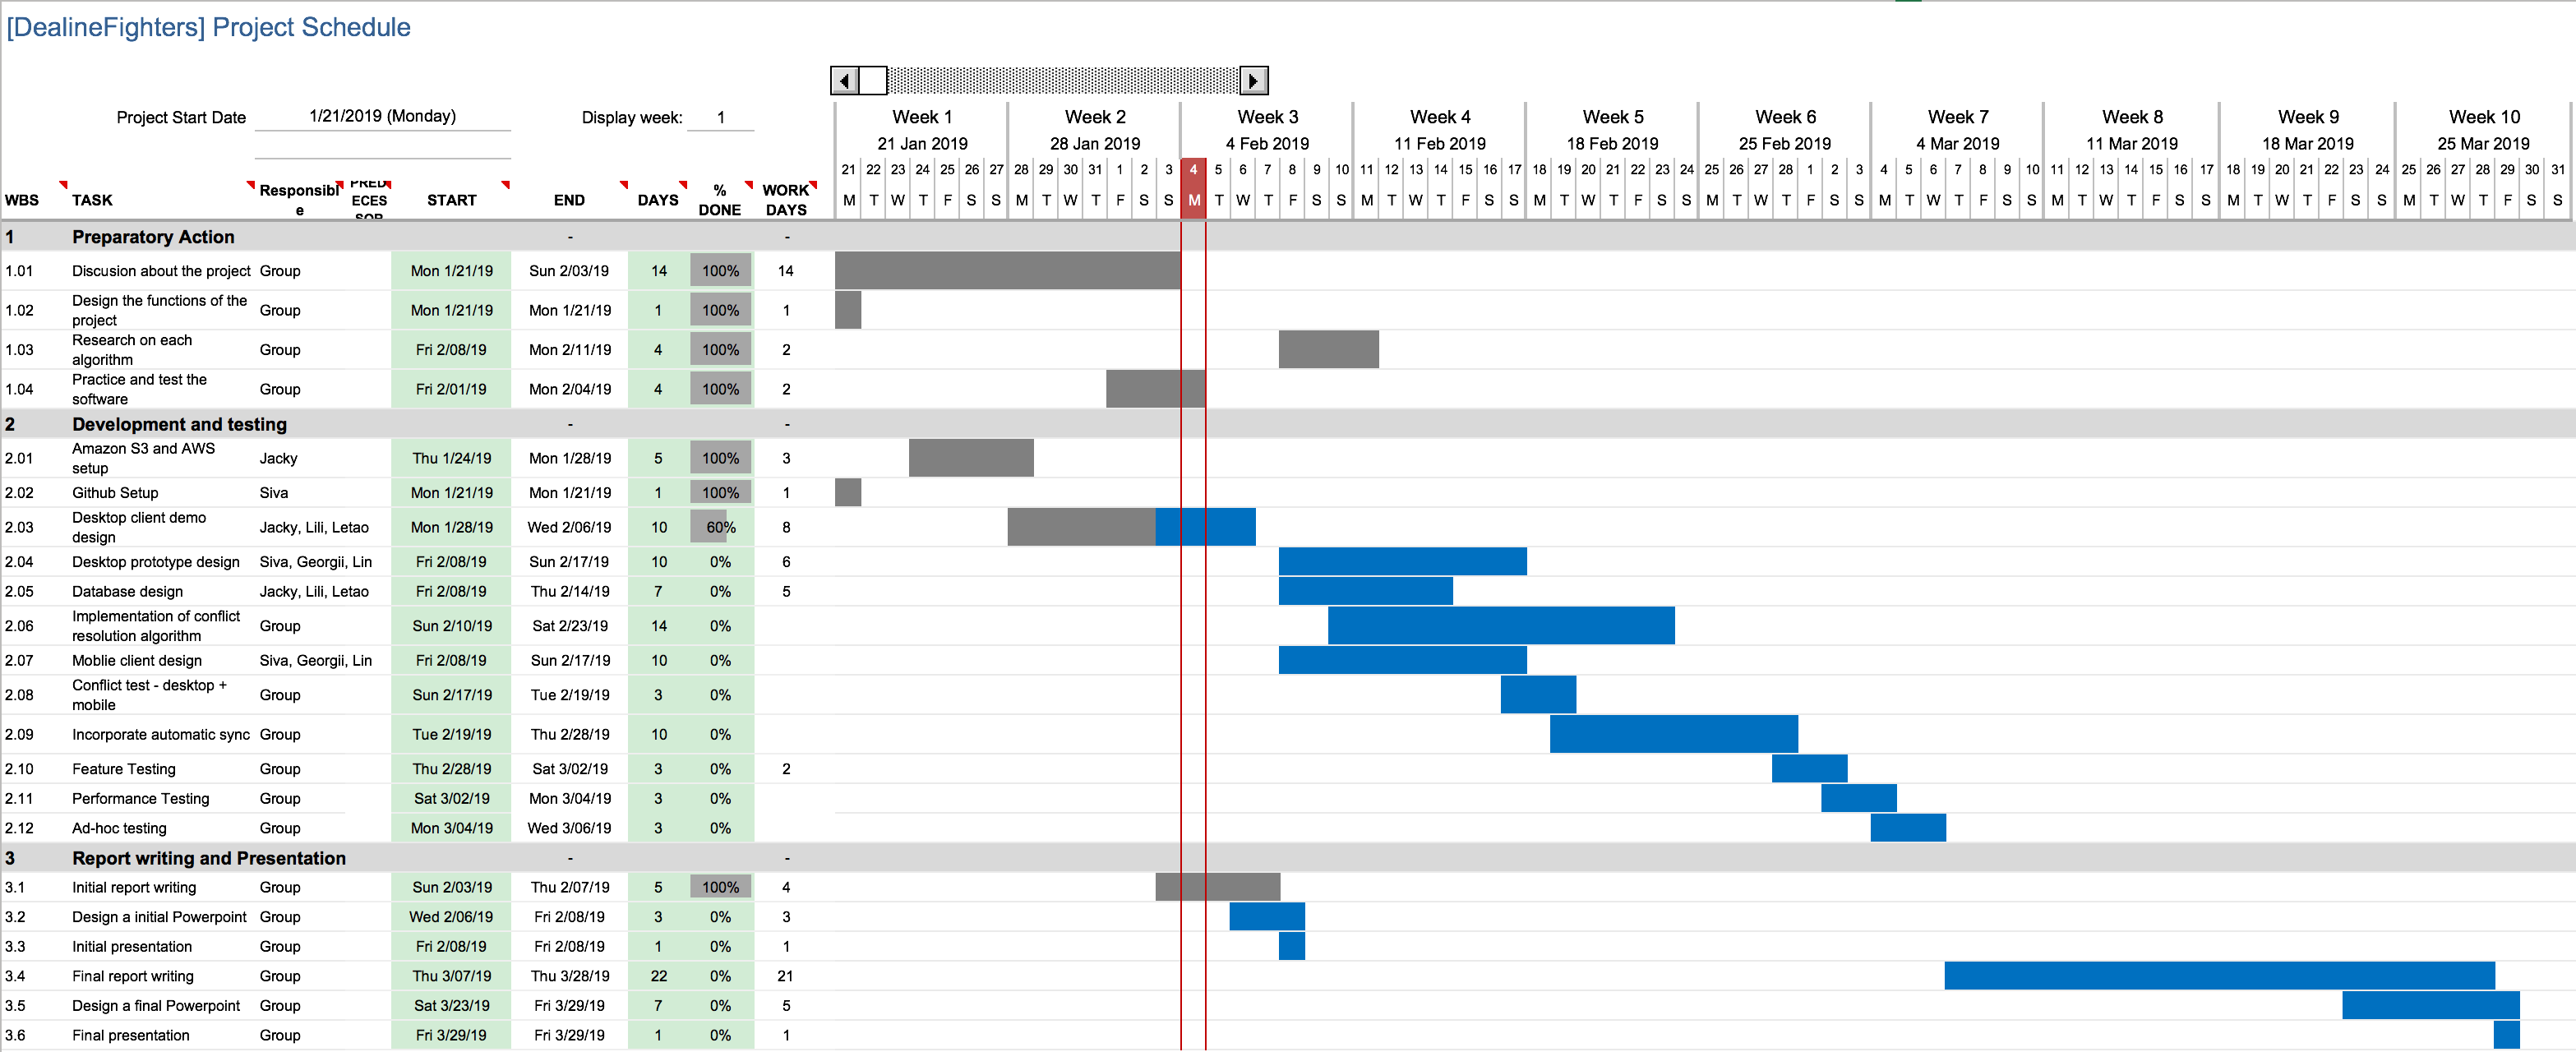
\includegraphics[scale=0.4]{Timeline_Ver_0}
\caption{This is Gantt chart which illustrates the plan of our group within 10 weeks.}
\end{sidewaysfigure}
}
\end{document}
